\begin{figure}
    \centering
    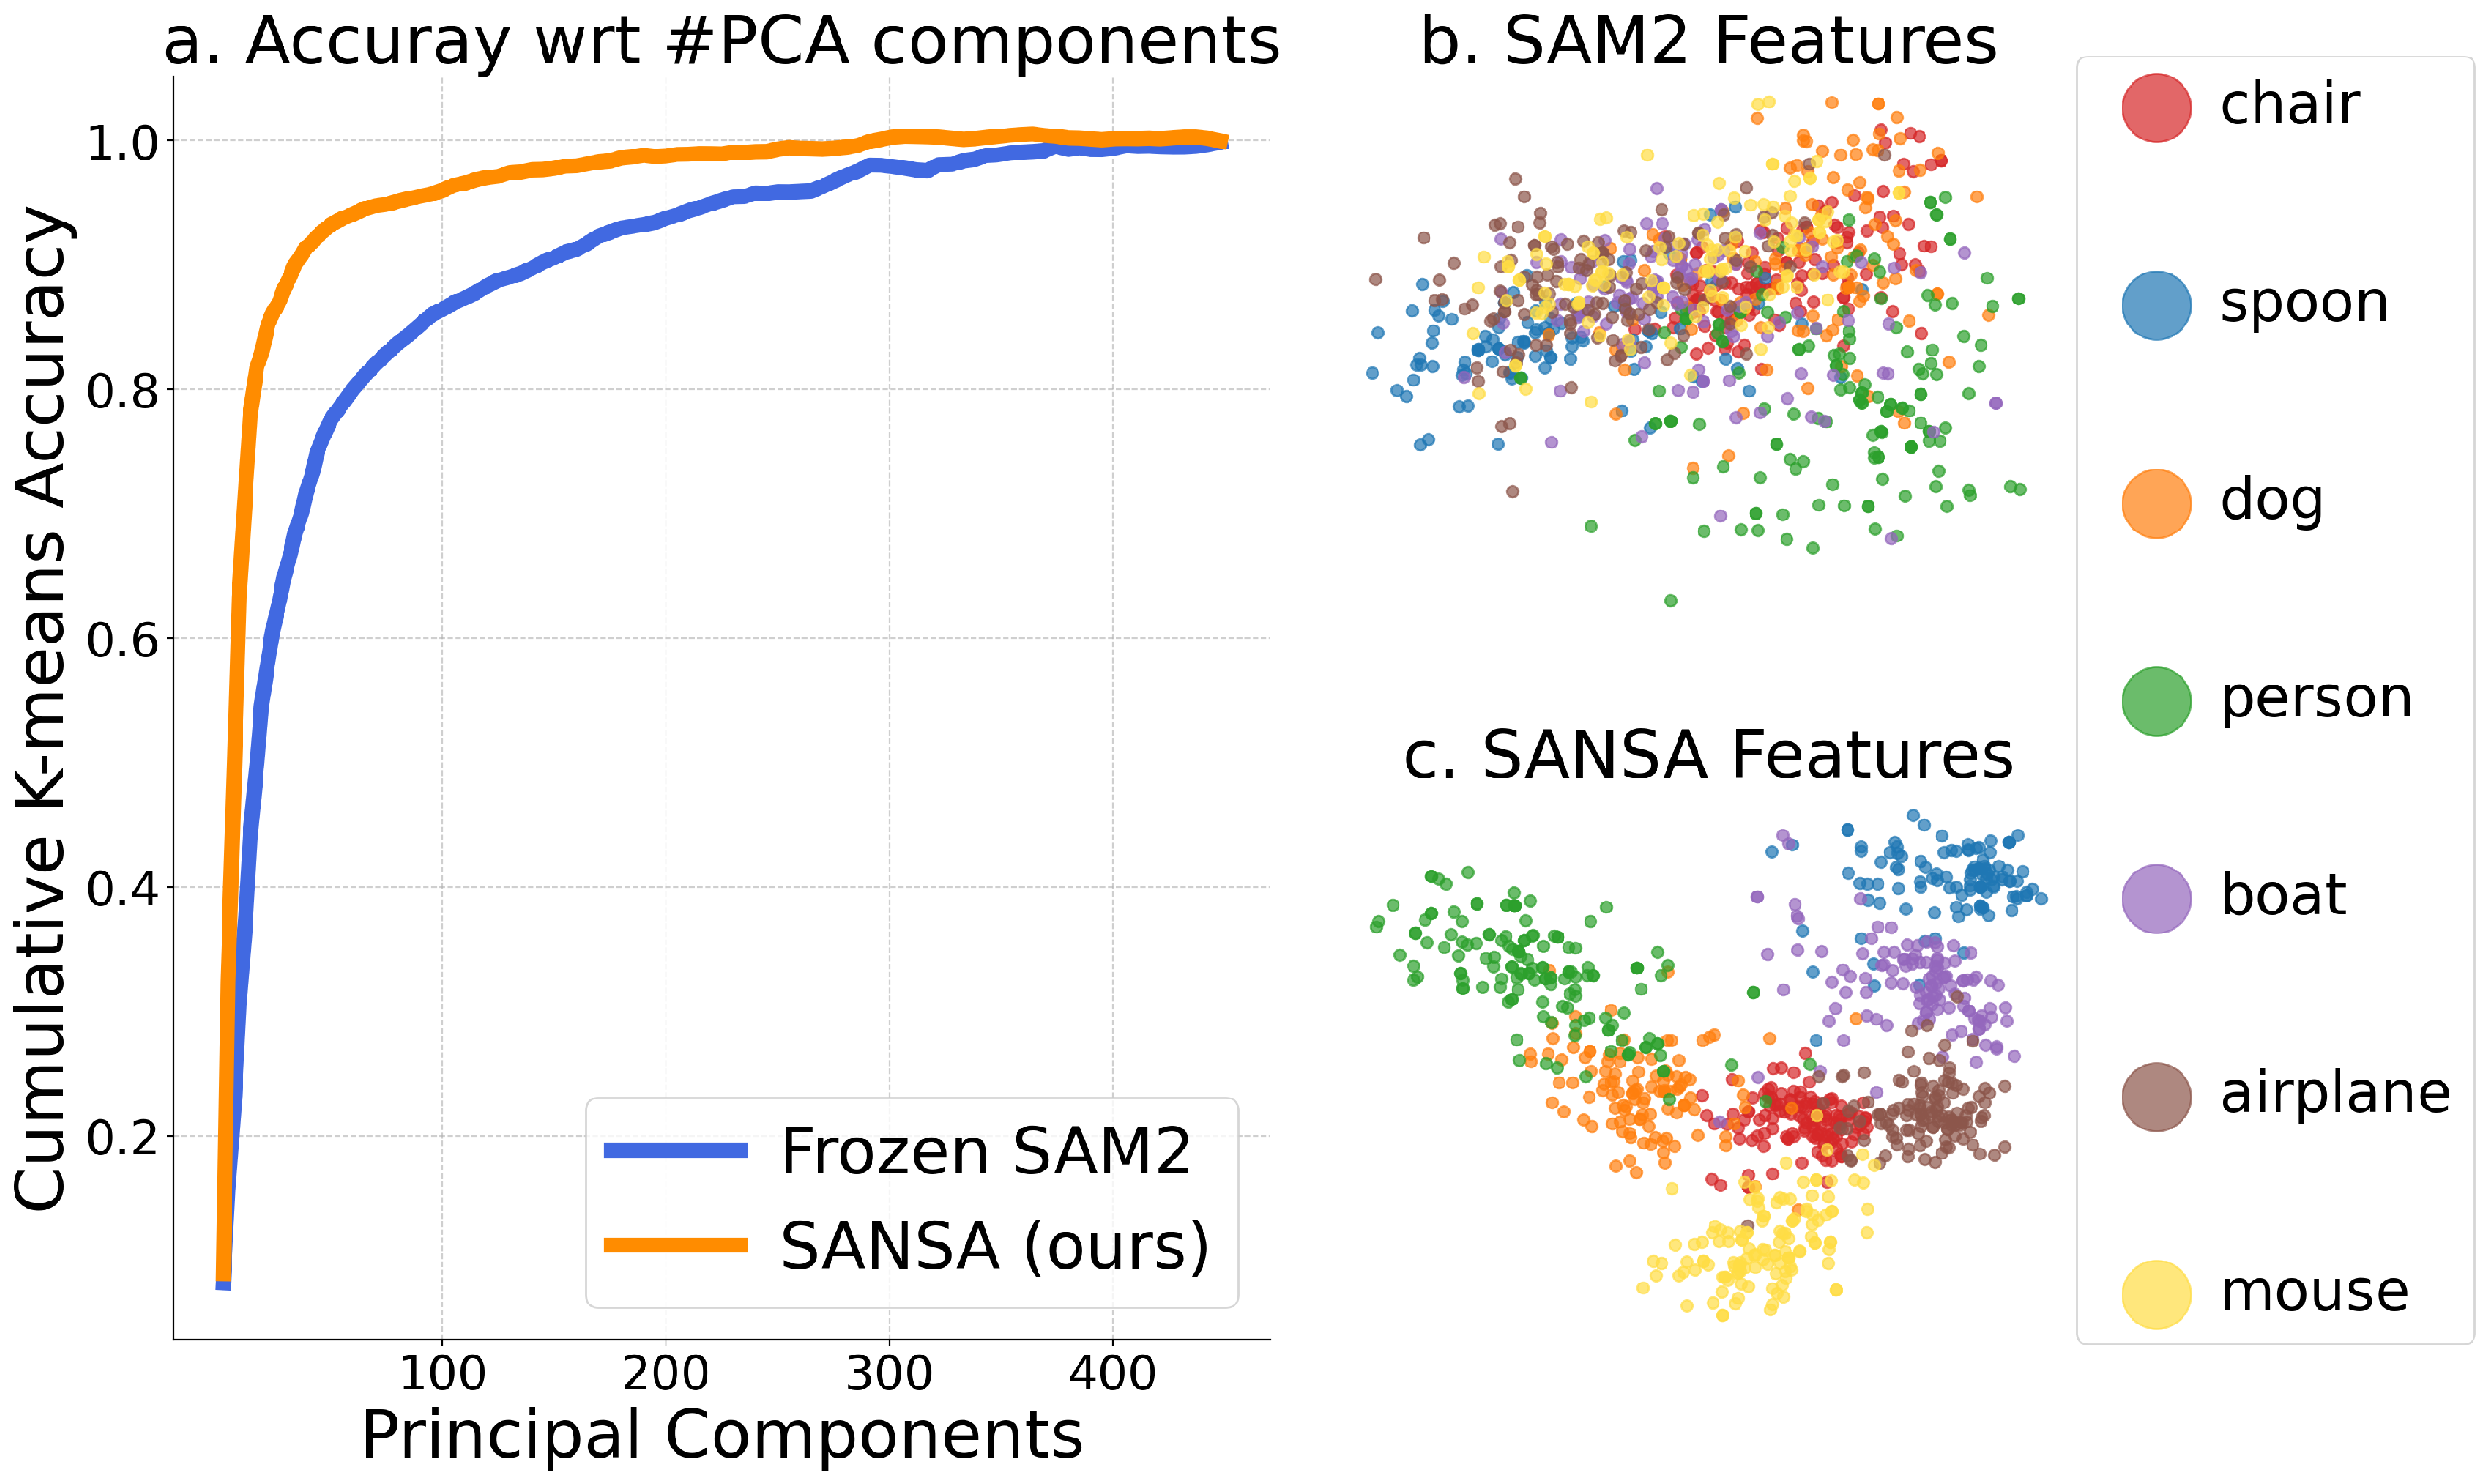
\includegraphics[width=.8\textwidth]{images/pca.pdf}
    \caption{\textbf{ Semantic information concentration across principal components.} (a) We evaluate how semantic information is distributed across the principal components of the feature space. For each number of retained components (x-axis), we compute class centroids on COCO-20$^i$ training embeddings and assign test embeddings to the nearest centroid. The y-axis shows the relative classification accuracy, normalized by the accuracy at full dimensionality. A steep rise (SANSA) indicates that semantic information is concentrated in the leading components; a gradual rise (SAM2) suggests it is  entangled with other signals.
    (b) 2D PCA projection of frozen SAM2 features, colored by class. Semantic structure is weak, with significant overlap across classes.
    (c) 2D PCA projection of SANSA features, showing compact and well-separated clusters aligned with semantic categories.
    }
\label{fig:pca}
\end{figure}
